\documentclass[12pt]{article}
\usepackage{amsmath}
\usepackage{gensymb}
\usepackage{float}
\usepackage[top=1.25in, bottom=1in, left=1in, right=1in]{geometry}
\usepackage{graphicx}
\usepackage[export]{adjustbox}
\usepackage{rotating}
\usepackage{multirow}
\usepackage{latexsym}
\usepackage{amssymb}
\usepackage{longtable}
\usepackage{fancyhdr}
\usepackage{color}
\usepackage{subcaption}
\usepackage{listings}
\usepackage{setspace}
\definecolor{Code}{rgb}{0,0,0}
\definecolor{Decorators}{rgb}{0.5,0.5,0.5}
\definecolor{Numbers}{rgb}{0.5,0,0}
\definecolor{MatchingBrackets}{rgb}{0.25,0.5,0.5}
\definecolor{Keywords}{rgb}{0,0,1}
\definecolor{self}{rgb}{0,0,0}
\definecolor{Strings}{rgb}{0,0.63,0}
\definecolor{Comments}{rgb}{0,0.63,1}
\definecolor{Backquotes}{rgb}{0,0,0}
\definecolor{Classname}{rgb}{0,0,0}
\definecolor{FunctionName}{rgb}{0,0,0}
\definecolor{Operators}{rgb}{0,0,0}
\definecolor{Background}{rgb}{0.98,0.98,0.98}
\lstdefinelanguage{Python}{
	numbers=left,
	numberstyle=\tiny ,
	numbersep=1em,
	xleftmargin=1em,
	framextopmargin=2em,
	framexbottommargin=2em,
	showspaces=false,
	showtabs=false,
	showstringspaces=false,
	frame=l,
	tabsize=4,
	% Basic
	basicstyle=\ttfamily\small\setstretch{1},
	%backgroundcolor=\color{Background},
	% Comments
	commentstyle=\color{Comments}\slshape,
	% Strings
	stringstyle=\color{Strings},
	morecomment=[s][\color{Strings}]{"""}{"""},
	morecomment=[s][\color{Strings}]{'''}{'''},
	% keywords
	morekeywords={import,from,class,def,for,while,if,is,in,elif,else,not,and,or,print,break,continue,return,True,False,None,access,as,,del,except,exec,finally,global,import,lambda,pass,print,raise,try,assert},
	keywordstyle={\color{Keywords}\bfseries},
	% additional keywords
	morekeywords={[2]@invariant,pylab,numpy,np,scipy},
	keywordstyle={[2]\color{Decorators}\slshape},
	emph={self},
	emphstyle={\color{self}\slshape},
	%
}

\definecolor{mygreen}{rgb}{0,0.6,0}
\definecolor{mygray}{rgb}{0.5,0.5,0.5}
\definecolor{mymauve}{rgb}{0.58,0,0.82}             
\pagestyle{fancy}
\fancyhf{}
\fancyhead[RE,RO]{Zixu Zhang\\zixu@umich.edu}
\fancyhead[LE,LO]{EECS 504\\FALL 2018 }
\fancyhead[C]{Homework 2\textsl{\textsl{}}}

\begin{document}
	\begin{enumerate}
	\item 
	\begin{enumerate}
	\item 
	Figure \ref{fig: 1aa} shows the corner response of checker board and Figure \ref{fig: 1ab} shows the actual corner detections after non-maximum suppression. The code is listed in appendix.
		\begin{figure}[H]
			\centering
			\begin{subfigure}[t]{0.5\textwidth}
				\centering
				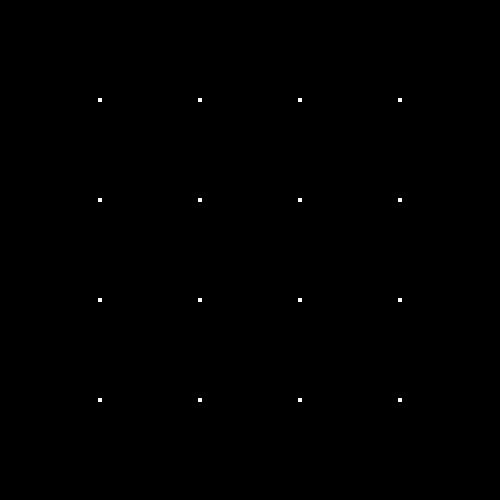
\includegraphics[width=\textwidth]{response_img.png}
				\caption{Checkerboard Response}
				\label{fig: 1aa}
			\end{subfigure}%
			~ 
			\begin{subfigure}[t]{0.5\textwidth}
				\centering
				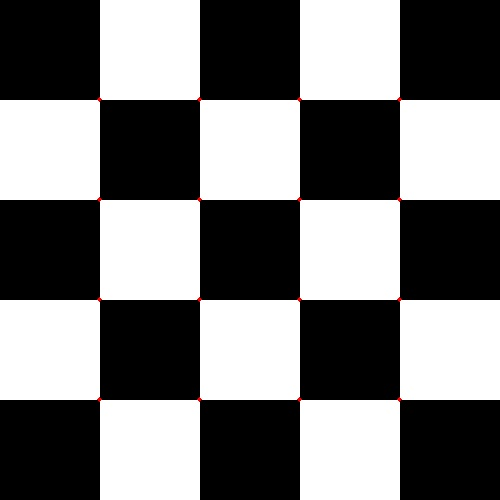
\includegraphics[width=\textwidth]{checkerboard_corners_after_sup.jpg}
				\caption{Actual Corner Detection}
				\label{fig: 1ab}
			\end{subfigure}
			\caption{Response matrix and corners of checkerboard}
		\end{figure}
	
	\item Figure \ref{fig: 1ba} shows the corner response of concentric circle and Figure \ref{fig: 1bb} shows the actual corner detections after non-maximum suppression. The code is listed in appendix.\\
	The results are obtained with half window size 2 and threshold 0.35. From those images, we can see that even it is a circle, there are a lot of high response region along edges of circles. One reason for those high response is that Harris corner detector focuses on local region where window covers. For low resolution image we use for this question, the circle's edge looks like steps. If we select a small size window, and construct a structure tensor based on that region. Eigenvalues may be relative large along both eigenvectors. Thus, this leads to false corners detection.\\
	On the other hand, high responses do not cover the whole ring. For example, at $0^\circ,\pm90^\circ,180^\circ$ positions of each ring, it is actually formed by straight lines. Trivially, corner response is weak along those line. Moreover For the $\pm 45^\circ $ and $\pm135^\circ$ positions of largest ring, and most of the second largest ring, corner response is also weak. That is because $I'_x$ and $I'_y$ are very close along those place, which leads to fairly small value for the smaller eigenvalue. Then the corner detector treats them as edges. 
	\begin{figure}[H]
		\centering
		\begin{subfigure}[t]{0.5\textwidth}
			\centering
			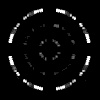
\includegraphics[width=\textwidth]{response_img_circle}
			\caption{Checkerboard Response}
			\label{fig: 1ba}
		\end{subfigure}%
		~ 
		\begin{subfigure}[t]{0.5\textwidth}
			\centering
			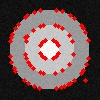
\includegraphics[width=\textwidth]{concentric_circles_corners_after_sup.jpg}
			\caption{Actual Corner Detection}
			\label{fig: 1bb}
		\end{subfigure}
		\caption{Response matrix and corners of checkerboard}
	\end{figure}
	\item The image stitching results with 4, 10 and 20 correspondence are shown in Figure \ref{fig 1c4}, \ref{fig 1c10}, and \ref{fig 1c20}. The code used for image stitching is listed in Appendix
	\begin{figure}[H]
		\centering
		\includegraphics[width=\textwidth]{stitched_image_4pts}
		\caption{Stitched images with 4 correspondences}
		\label{fig 1c4}
	\end{figure}
	As we can see that stitching with only 4 points fails completely. To investigate the reason of failure, we plot out the corresponding points in original images as Figure \ref{fig: 1c_corr}. We can see that all four points lies in a small region of both images, this makes the estimated homography not general enough to represent the 2D projective transformations of the entire image. Moreover, if we look at the processes of least square estimation, there are 8 parameters in the homograph matrix. With only 4 points, the estimated homograph will leads to error $\eta=0$ for least square. In this way, a small error in the location of correspondent pixel will cause big change in the estimated homography.\\
	Thus, to improve the results of stitching, increasing number of correspondence should be used. 
	\begin{figure}[H]
		\centering
		\adjincludegraphics[width=\textwidth,trim={{.1\width} {.3\height} {.1\width} {.3\height}},clip,]{q1c_corres.eps}
		\caption{4 correspondences in left and right images}
		\label{fig: 1c_corr}
	\end{figure}

\item We tested image stitching with 10 and 20 correspondences as shown in Figure \ref{fig 1c10} and \ref{fig 1c20}. We can see that there are tremendous improvement of stitching as the number of correspondence increase from 4 to 10 and 20.
\begin{figure}[H]
	\centering
	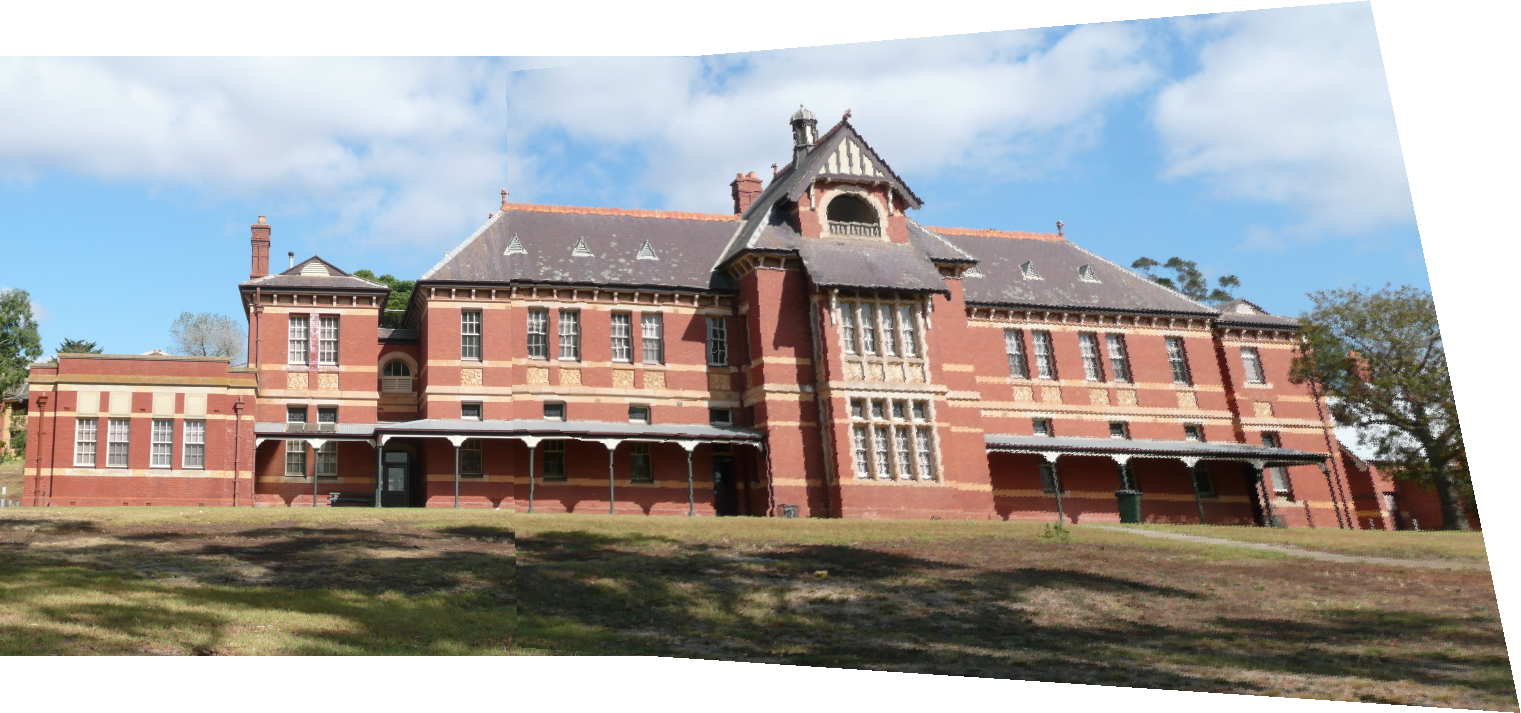
\includegraphics[width=\textwidth]{stitched_image_10pts}
	\caption{Stitched images with 10 correspondences}
	\label{fig 1c10}
\end{figure}
\begin{figure}[H]
	\centering
	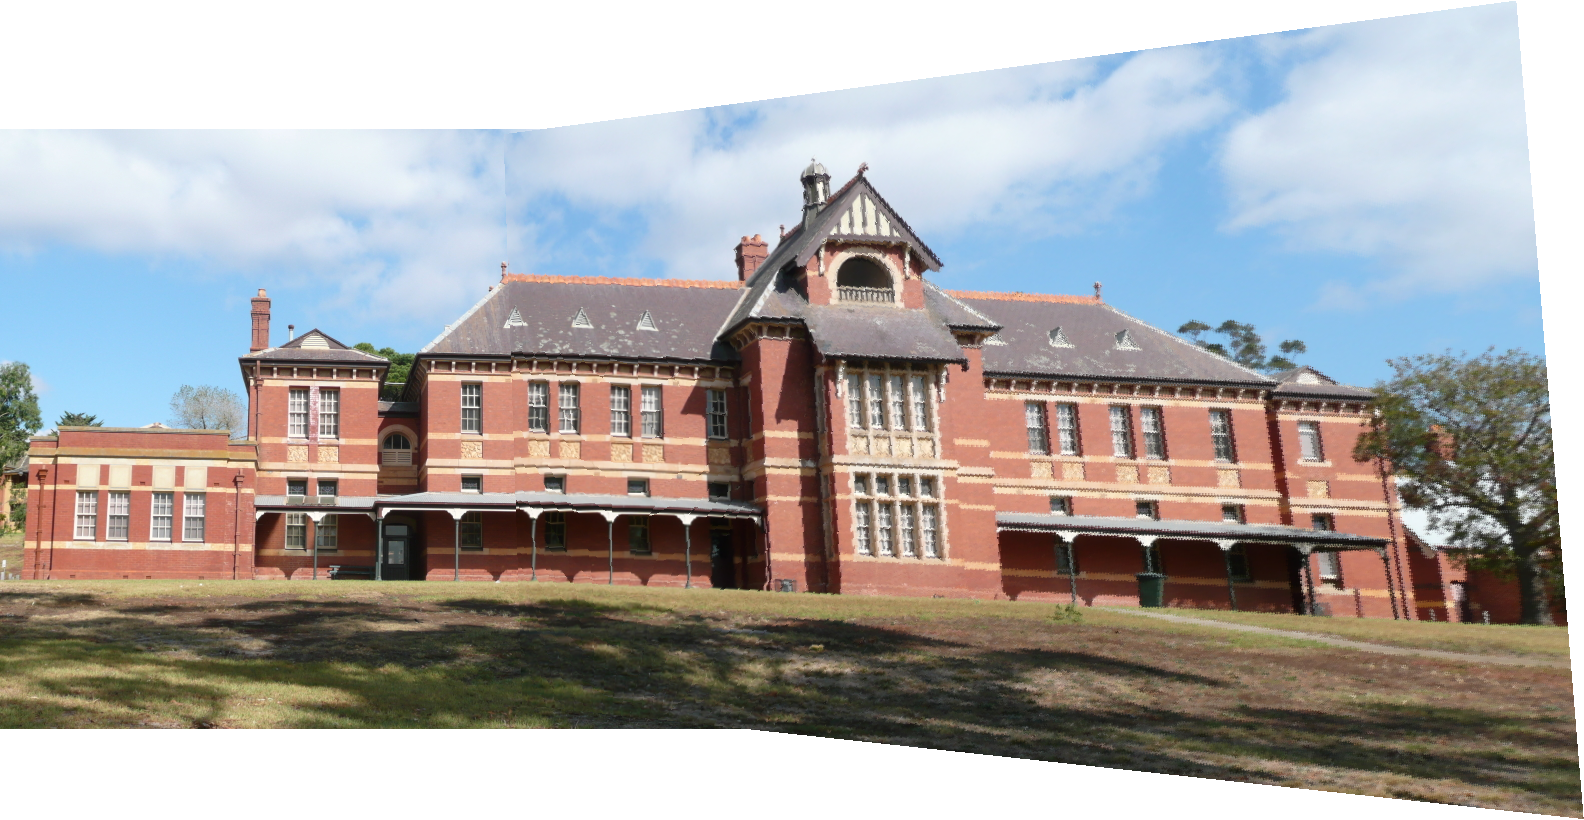
\includegraphics[width=\textwidth]{stitched_image_20pts}
	\caption{Stitched images with 20 correspondences}
	\label{fig 1c20}
\end{figure}
As we have explained in previous question. Top 4 correspondences are in a small region of both images, and they are not robust to errors in pixel locations of correspondence. Instead, if we use top 10 correspondences, points are more evenly distributed in the overlap region of both images. Thus, the estimated homography is much better and overdetermined system is also more robust to errors in pixel correspondences.\\
20 points of correspondences also provide us a fairly good stitching. Compared with 10 correspondences, all vertical edges in the right (stitched) image are better aligned with vertical edges in the left (basis) image. Moreover, we can see that the ground in the 20 correspondences result is better stitched than 10 correspondences. On the other hand, we find 20 correspondences result is worse stitched at building region. For example, if we look at the canopy, which is perfectly aligned in 10 correspondences but misaligned in 20. This is because 20 correspondences use those weaker features that have relatively large error of matching.

 

	\end{enumerate}
	\pagebreak
	\item 
	\begin{enumerate}
		\item All non-horizontal and non-vertical edges of the image is shown in Figure \ref{fig: 1a}. The code is listed in appendix.
		\begin{figure}[H]
			\centering
			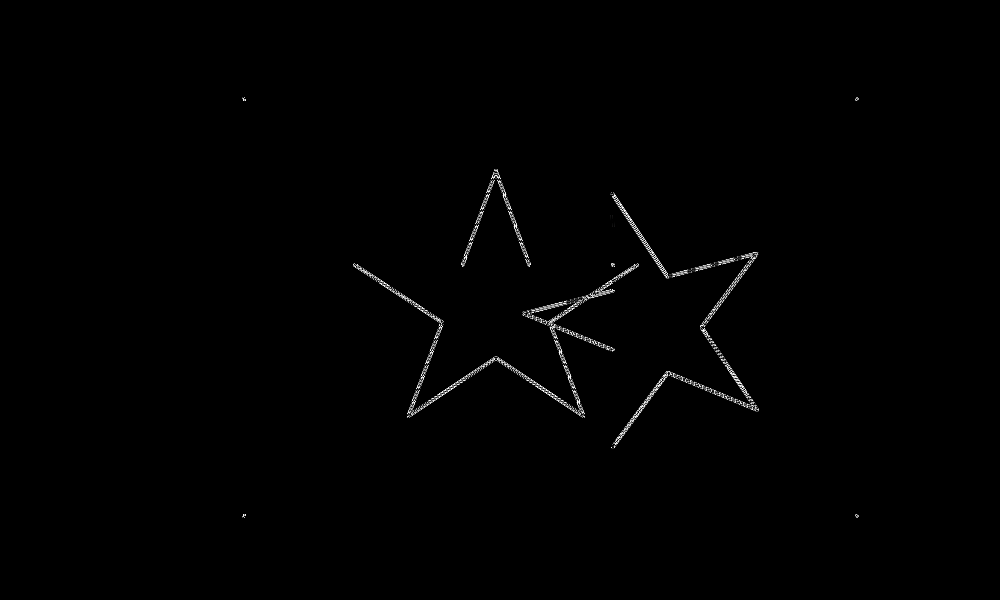
\includegraphics[width=\textwidth]{steerable_filter_output}
			\caption{non-horizontal and non-vertical edges}
			\label{fig: 1a}
		\end{figure}
	
	\item Yes, first-order derivative of 2-D Gaussian filter is steerable.\\
	Proof: If we consider the continuous case of Gaussian filter with $\sigma =1$ and ignore the scaling constant $\frac{1}{\sqrt{2\pi\sigma^2}}$
	$$g(x,y) = \exp(-\frac{x^2+y^2}{2})$$
	$$\frac{\partial}{\partial x}g(x,y) = -x\exp(-\frac{x^2+y^2}{2}),~\frac{\partial}{\partial y}g(x,y) = -y\exp(-\frac{x^2+y^2}{2})$$
	If we convert $x,~y$ into polar coordinate, such that $x=r\cos\theta$ and $y=r\sin\theta$
	$$g_x(r,\theta) = -r\cos\theta\exp(-r^2/2),~g_y(r,\theta)=-r\sin\theta\exp(-r^2/2)$$
	If we say that we want to take derivative of this Gaussian filter in arbitrary orientation $\hat{i}$ by rotate the $\hat{x}$ by $\alpha$ degree,
	$$\hat{i} = r\cos(\theta-\alpha)$$  
	$$g_{\hat{i}}(r,\theta) =\frac{\partial g(r,\theta)}{\partial (r\cos(\theta-\alpha))}=\frac{\partial}{\partial (r\cos(\theta-\alpha))}\exp(-\frac{(r\cos(\theta-\alpha))^2+(r\sin(\theta-\alpha))^2}{2}$$ $$=-r\cos(\theta-\alpha)\exp(-r^2/2)$$
	$$=-r\exp(-r^2/2)(\cos\theta\cos\alpha+\sin\theta\sin\alpha)$$
	$$=\begin{bmatrix}
	\cos\alpha& \sin\alpha
	\end{bmatrix}\begin{bmatrix}
	-r\exp(-r^2/2)\cos\theta\\
	-r\exp(-r^2/2)\sin\theta
	\end{bmatrix}$$
	$$=\begin{bmatrix}
	\cos\alpha& \sin\alpha
	\end{bmatrix}\begin{bmatrix}
	g_x\\
	g_y
	\end{bmatrix}$$
	Since the covariance $\sigma$ will not affect any transformation above, we can conclude that for a Gaussian filter $g(x,y,\sigma)=\exp(-\frac{x^2+y^2}{2\sigma^2})$, its derivative with respect of an arbitrary orientation $\hat{i}$, which rotate $\alpha$ from $x$-axis can be expressed as the linear combination:
	$$g_i(x,y,\sigma) = g_i(r,\theta,\sigma)=\begin{bmatrix}
	\cos\alpha& \sin\alpha
	\end{bmatrix}\begin{bmatrix}
	g_x(x,y,\sigma)\\
	g_y(x,y,\sigma)
	\end{bmatrix}$$
	From our definition, we can see that first derivate of Gaussian filter is steerable, with basis function $\begin{Bmatrix}
	g_x(x,y,\sigma)&
	g_y(x,y,\sigma)
	\end{Bmatrix}$. \\
	
	\item Yes. Dimension of the basis is three. First, we define the Fourier transform of 2D Gaussian $g(x,y)$ as $G(w_x,w_y)$, such that by the property of Fourier transform,$n$-th derivative of 2D Gaussian $g(x,y)$ along $x$-axis is $g^{(n)}_x(x,y)$ and its Fourier transform is $$G^{(n)}_x(w_x,w_y)=(-j\begin{bmatrix}
	w_x&w_y
	\end{bmatrix}\begin{bmatrix}
		1\\0
		\end{bmatrix})^nG(w_x,w_y)$$
		Generally speaking, if we take the second derivative along an arbitrary axis $\hat{u}=\begin{bmatrix}\cos\alpha &\sin\alpha \end{bmatrix}^T$,
		 $$G^{(n)}_{\hat{u}}(w_x,w_y)=(-j\begin{bmatrix}
		 w_x&w_y
		 \end{bmatrix}\hat{u})^nG(w_x,w_y)$$
		 Thus, we can say that 
		$$G^{(2)}_{\hat{u}}(w_x,w_y) = (
		w_x\cos\alpha +w_y\sin\alpha)^2G(w_x,w_y)$$
		By the binomial theorem as
		$$(a+b)^n = \sum_{k=0}^n { {n}\choose{k}}a^{3-k}b^k$$
		We can see that $G^{(2)}_{\hat{u}}(w_x,w_y)$ is the sum of 3 distinct element in Fourier. Thus, we can convert it back to spatial domain and $g^{(n)}_{\hat{u}}(x,y)$ is the linear combination of 3 distinct basis.\\
		We can also apply previous steps to higher dimension. We can conclude that $n$-th derivative of 2D Gaussian is a steerable filter with $n+1$ dimension basis.
	\end{enumerate}

		\item 
		\begin{enumerate}
			\item With image size $n\times n$ and kernel size $2k+1\times2k+1$, the output of this convolution is $n-2k\times n-2k$. For each iteration of convolution, it needs $(2k+1)^2$ times multiplications and $(2k+1)^2$ times addition. Thus, the total number of operations in term of multiplies and adds is $2(2k+1)^2(n-2k)^2$.\\
			
			\item Consider a 2D Gaussian filter $g(x,y)=\frac{1}{2\pi\sigma^2}\exp(-\frac{x^2+y^2}{2\sigma^2})$. It is equal to $g(x)g(y)=\frac{1}{\sqrt{2\pi\sigma^2}}\exp(-\frac{x^2}{2\sigma^2})\frac{1}{\sqrt{2\pi\sigma^2}}\exp(-\frac{y^2}{2\sigma^2})$. In discrete case, we can write the kernel $G_2\in\mathbb{R}^{2k+1\times2k+1}=G_1^TG_1$, where $G_1\in\mathbb{R}^{1\times2k+1}$ is a 1D Gaussian kernel in horizontal direction, and $G_1^T$ is the same 1D Gaussian kernel in vertical direction.
			$$(I*G_2)[x,y]=\sum_{j=-k}^k\sum_{i=-k}^kI(x-i,y-j)G_2(i,j)$$
			$$\because G_2(i,j)=G_1^T(i)G_1(j)$$
			$$(I*G_2)[x,y] = \sum_{j=-k}^k\sum_{i=-k}^kI(x-i,y-j)G_1^T(i)G_1(j)$$
			$$=\sum_{j=-k}^kG_1(j)\sum_{i=-k}^kI(x-i,y-j)G_1^T(i)$$
			$$\because(I*G_1^T)[x,y-j]= \sum_{i=-k}^kI(x-i,y-j)G_1^T(i)$$
			$$\therefore (I*G_2)[x,y] = \sum_{j=-k}^kG_1(j)(I*G_1^T)[x,y-j]=(I*G_1^T*G_1)$$
			Therefore, since 2D Gaussian kernel can be expressed by the vector multiplication of a vertical and a horizontal 1D Gaussian kernels with same covariance, the convolution of an image with a 2D Gaussian filter can be reduced by a sequential convolution with a vertical and a horizontal 1D Gaussian kernels.\\
			
			\item First convolution $I*G_1^T$, the resultant matrix has size $(n-2k)\times n$. At each window, it requires $(2k+1)$ multiplications and $(2k+1)$ additions. In total, $2(2k+1)(n-2k)n$ operations during the first operation.\\
			Second convolution $(I*G_1^T)*G_1$, the final output matrix has size $(n-2k)\times(n-2k)$. At each window, it also needs $(2k+1)$ multiplications and $(2k+1)$ additions. In total, $2(2k+1)(n-2k)(n-2k)$ operations during the second operation.\\
			After two sequential convolutions, there are $2(2k+1)(n-2k)(2n-2k)$ operations in total.\\
			
			\item No. 2D Laplacian kernel cannot be separated to 1D kernels.\\
			 If a 2D kernel $H\in\mathbb{R}^{2k+1\times 2k+1}$ is able to be separable to 1D kernels $f\in\mathbb{R}^{2k+1\times1}$ and $g\in\mathbb{R}^{1\times2k+1}$, we should be able to find $H=fg$. Which means, every row of $H$ is a multiplicity of others. However, if we look at the Laplacian kernel:
			 $$LoG(x,y) = -\frac{1}{\pi\sigma^4} (1-\frac{x^2+y^2}{2\sigma^2})\exp(-\frac{x^2+y^2}{2\sigma^2})$$
			 If we look different $x_1$ and $x_2$, it is easily to see that there does not exist a constant $\epsilon$, such that $LoG(x_1,y)=\epsilon LoG(x_2,y), \forall y$. Therefore, 2D Laplacian kernel cannot be separated to 1D kernels. 
		\end{enumerate}
	\end{enumerate}
	
	
	
	
	
	
	
	
	\pagebreak
	\textbf{Appendix:}
\begin{lstlisting}[language=python]
def _get_harris_corner(Gx, Gy, window_half_size, threshold):
	height, width = Gx.shape
	 #initialize corner_location_matrix 0x2
	corner_location_matrix = np.array([[],[]]).T
	 #initialize corner_response_matrix 
	corner_response_matrix = np.zeros([height,width])
	
	#get Gx^2, Gy^2, GxGy
	Gx2 = np.multiply(Gx,Gx) #Ix^2(y,x)
	Gy2 = np.multiply(Gy,Gy) #Iy^2(y,x)
	Gxy = np.multiply(Gx,Gy) #I_xy(y,x)
	
	#Use a (2k+1)*(2k+1) summing filter to get summation
	kernel_sum = np.ones([window_half_size*2+1,window_half_size*2+1])
	sum_Gx2 = signal.convolve2d(Gx2, kernel_sum, mode='valid')
	sum_Gy2 = signal.convolve2d(Gy2, kernel_sum, mode='valid')
	sum_Gxy = signal.convolve2d(Gxy, kernel_sum, mode='valid')
	for i in range(sum_Gx2.shape[0]):
		for j in range(sum_Gx2.shape[1]):
			structureTensor = np.array([[sum_Gx2[i,j], 
				sum_Gxy[i,j]],[sum_Gxy[i, j], sum_Gy2[i, j]]])
			eigVal = np.linalg.eigvals(structureTensor)
			minEig = min(eigVal)
			# check if the lambda_2 is larger than threshold
			if minEig > threshold:
				corner_response_matrix[i+window_half_size,
					 j+window_half_size] = minEig
				cur_loc = np.array([[j+window_half_size,
					i+window_half_size]])
				corner_location_matrix = np.append(
					corner_location_matrix, cur_loc, axis=0)
	return corner_response_matrix, corner_location_matrix
\end{lstlisting}
\pagebreak
\begin{lstlisting}[language=python]
def _get_homography(img1_keypoints, img2_keypoints):
	homog_matrix = np.zeros((3,3))
	num_corres = len(img1_keypoints)
	yVec = np.ones((2*num_corres)) # vector y
	aMat = np.zeros((2*num_corres,8)) # Matrix A
	for i in range(num_corres): 
	'''form matrix a and y for LR'''
		yVec[2*i] = img1_keypoints[i][0]
		yVec[2*i+1] = img1_keypoints[i][1]
		aMat[2*i, 0:2] = img2_keypoints[i]
		aMat[2*i, 2]=1
		aMat[2*i,6:8] = -img1_keypoints[i][0]*img2_keypoints[i]
		aMat[2*i+1, 3:5] = img2_keypoints[i]
		aMat[2*i+1, 5]=1
		aMat[2*i+1,6:8] = -img1_keypoints[i][1]*img2_keypoints[i]
	'''solve for x*=argmin||Ax-y||_2'''
	xVec = np.matmul(np.matmul(np.linalg.inv((np.matmul(aMat.T,aMat))),
			aMat.T),yVec)
	homog_matrix[0,:] = xVec[0:3]
	homog_matrix[1,:]=xVec[3:6]
	homog_matrix[2,0:2]=xVec[6:8]
	homog_matrix[2,2] = 1
	return homog_matrix

\end{lstlisting}
\vspace{3em}
\begin{lstlisting}[language=python]
def _bilinear_interpolation(x, y, pixel_mat, x1, y1, x2, y2):
	x_diff = np.array([[x2-x, x-x1]])
	y_diff = np.array([[y2-y],[y-y1]])
	if len(pixel_mat.shape)==3: #rgb case
		interpolation = np.zeros((1,1,3))
		for i in range(3):
			interpolation[:,:,i] = np.matmul(np.matmul(x_diff, 
				pixel_mat[:,:,i]),y_diff)/((x2-x1)*(y2-y1))
	else:
		interpolation = np.matmul(np.matmul(x_diff, pixel_mat),
			y_diff)/((x2-x1)*(y2-y1))
	return interpolation

def _overlap(img1, img2, homog_matrix):
	                  
	if len(img1.shape)>2: #RGB img
		img1_height, img1_width, num_ch1 = img1.shape
		img2_height, img2_width, _ = img2.shape
	else: #grayscale img
		num_ch1 =1
		img1_height, img1_width = img1.shape
		img2_height, img2_width = img2.shape
	
	'''create max/min pixel location matrix in homogenous coordindates'''
	locMat = np.array([[0, 0, img2_width-1, img1_width-1], 
		[0, img1_height-1, 0, img1_height-1], [1,1,1,1]])
	'''apply homography to the img2's pixel location'''
	locMat_trans_homo = np.matmul(homog_matrix, locMat)
	locMat_trans = np.round(locMat_trans_homo[0:2,:]/locMat_trans_homo[2,:])
	T_inv = np.linalg.inv(homog_matrix)
	'''find the size of new image'''
	min_x = int(min(0, np.amin(locMat_trans[0])))
	min_y = int(min(0, np.amin(locMat_trans[1])))
	max_x = int(max(img1_width-1, np.amax(locMat_trans[0])))
	max_y = int(max(img1_height-1, np.amax(locMat_trans[1])))
	
	new_img_height = max_y-min_y+1
	new_img_width = max_x-min_x+1
	if num_ch1 ==1: #grayscale
		out_img = np.zeros((new_img_height, new_img_width))
		''' map img1 to output img'''
		out_img[(-min_y):(img1_height-min_y),
			(-min_x):(img1_width-min_x)] = img1
		''' map img2 to stitched img'''
		for i in range(new_img_height):
			for j in range(new_img_width):
				temp_x_p = np.array([[j+min_x, i+min_y, 1]]).T
				temp_x = np.matmul( T_inv , temp_x_p)
				x_int = temp_x[0,0]/temp_x[2,0]
				y_int = temp_x[1,0]/temp_x[2,0]
				if 0<=x_int and x_int<img2_width-1 
					and 0<=y_int and y_int<img2_height-1:
					x1_int = np.floor(x_int)
					x2_int = x1_int+1
					y1_int = np.floor(y_int)
					y2_int = y1_int+1
					pixel_mat = img2[int(y1_int):int(y2_int)+1 ,
						 int(x1_int):int(x2_int)+1]
					interpolation = _bilinear_interpolation(x_int,
						y_int,pixel_mat,x1_int,y1_int,x2_int,y2_int)
					out_img[i,j] = interpolation.astype(int)
	else: #RGB case
		out_img = 255*np.ones((new_img_height, new_img_width, num_ch1))
		''' map img1 to output img'''
		out_img[(-min_y):(img1_height-min_y),(-min_x):(img1_width-min_x), :] = img1
		''' map img2 to stitched img'''
		
		for i in range(new_img_height):
			for j in range(new_img_width):
				temp_x_p = np.array([[j+min_x, i+min_y, 1]]).T
				temp_x = np.matmul( T_inv , temp_x_p)
				x_int = temp_x[0,0]/temp_x[2,0]
				y_int = temp_x[1,0]/temp_x[2,0]
				if 0<=x_int and x_int<img2_width-1 
					and 0<=y_int and y_int<img2_height-1:
					x1_int = np.floor(x_int)
					x2_int = x1_int+1
					y1_int = np.floor(y_int)
					y2_int = y1_int+1
					pixel_mat = img2[int(y1_int):int(y2_int)+1,
						 int(x1_int):int(x2_int)+1,:]
					interpolation = _bilinear_interpolation(x_int,y_int,
						pixel_mat,x1_int,y1_int,x2_int,y2_int)
					out_img[i,j,:] = interpolation.astype(int)
	return out_img
\end{lstlisting}
\vspace{3em}
\begin{lstlisting}[language=python]
def _apply_steerable_filter(G_x, G_y):
	g_intensity = np.empty_like(G_x)
	Gx2 = G_x*G_x
	Gy2 = G_y*G_y
	mask = np.ones_like(G_x)
	orientation = np.rad2deg(np.arctan2(G_y,G_x))
	loc =( ((-5<=orientation) & (orientation<=5)) 
		| ((85<=orientation) & (orientation<=95)) 
		| ((-95<=orientation) & (orientation<=-85)) 
		| (175<=orientation) | (orientation<=-175)).nonzero() 
	
	mask[loc] = 0
	g_intensity = (np.sqrt((Gx2+Gy2)*mask)).astype(np.uint8)
	#sio.savemat('/home/zixu/steerable.mat',dict([('Gx',G_x),('Gy',G_y),('g_intensity',g_intensity),('orientation',orientation)]))
	return g_intensity
\end{lstlisting}

\end{document}